\chapter{Guía de usuario}

Este capítulo se plantea como una guía de cara a un usuario final que tenga que usar la cinta transportadora presente en el laboratorio de Automática de la ETSI. Está pensado para ser leído independientemente del resto del trabajo sin conocimientos previos.

\section{Descripción y cuadro de mandos}

Este panel de control se trata de una interfaz que es capaz de mover la cinta transportadora y enviar la posición de una pieza 

\begin{figure}[htbp]
	\centering
	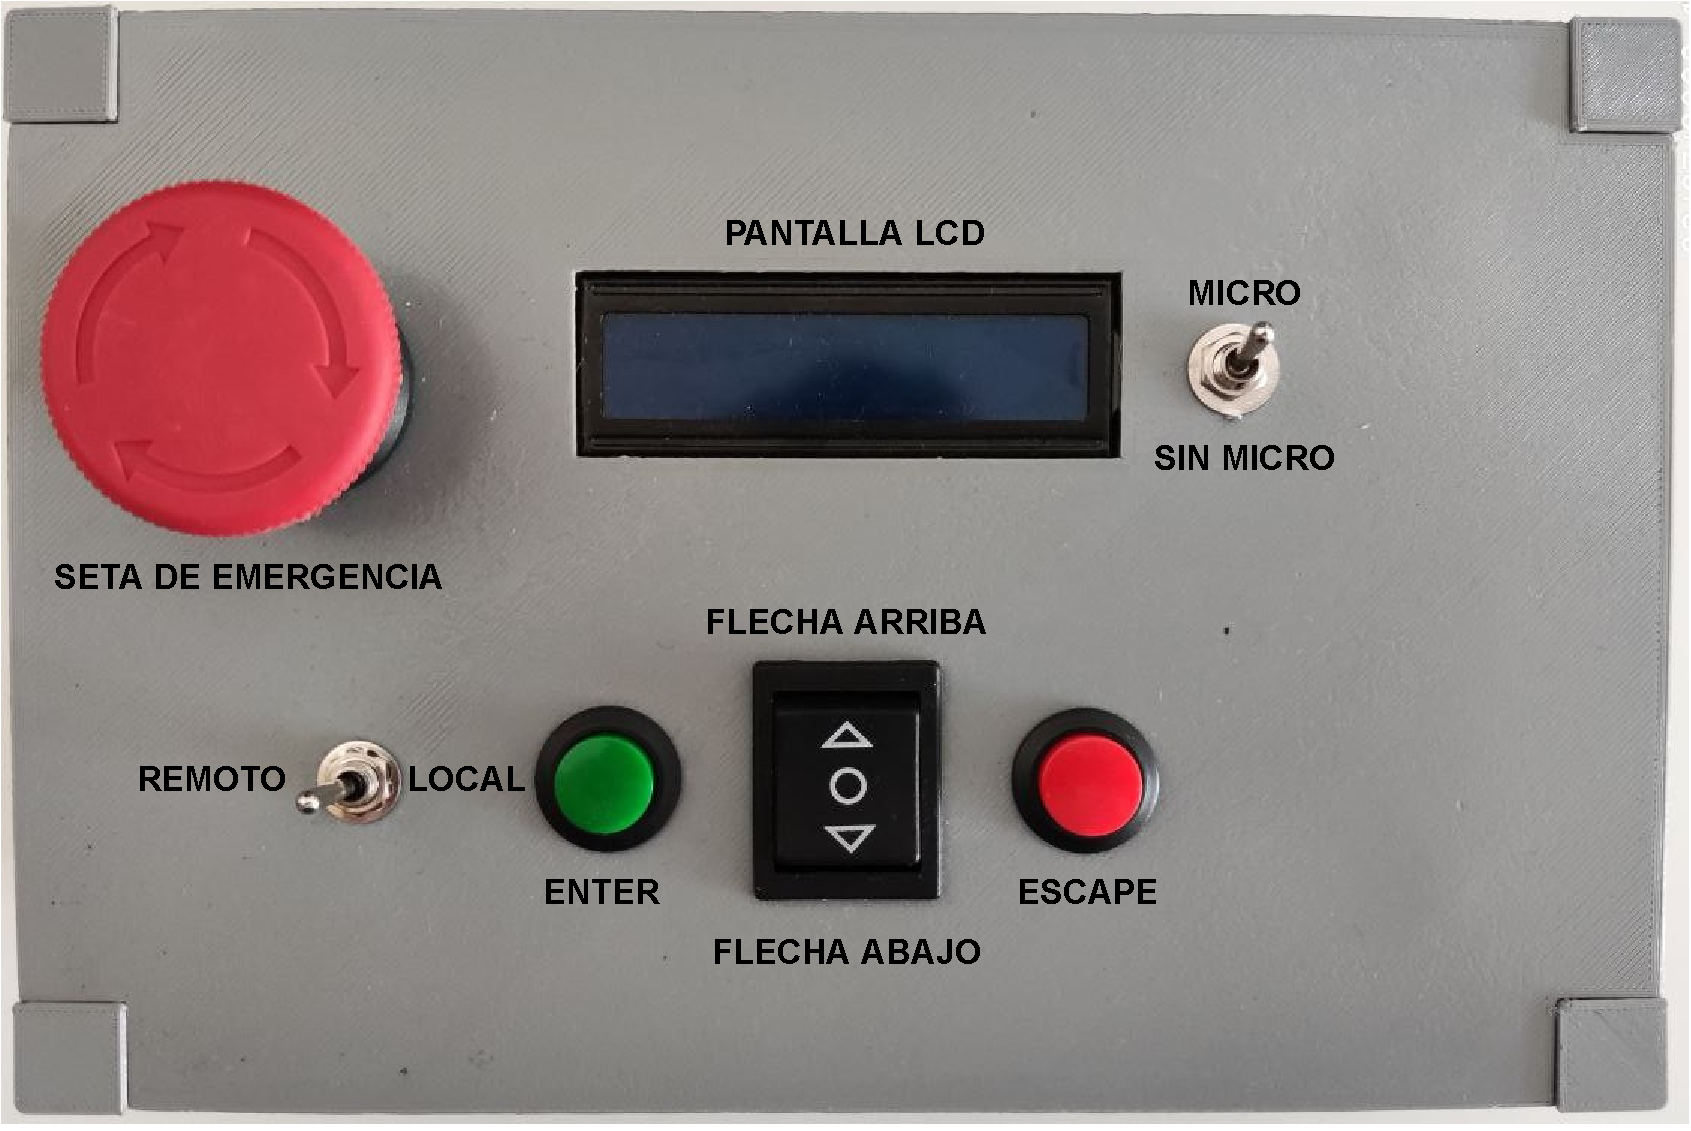
\includegraphics[width=\textwidth]{09-guiadeuso/HMI_REAL.pdf}
	\caption{Comandos del panel de control}
	\label{fig:interfazhmireal}
	\end{figure}



    \begin{figure}[htbp]
        \centering
        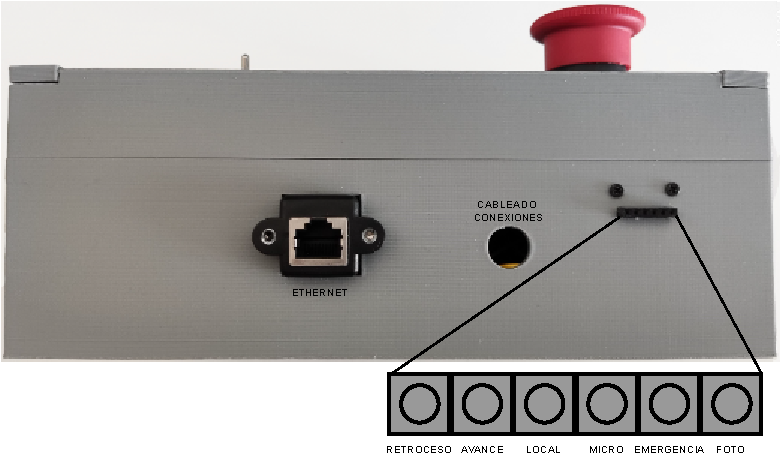
\includegraphics[width=\textwidth]{09-guiadeuso/DIGITALES_REAL.pdf}
        \caption{}
        \label{fig:pinesdigitalesreal}
        \end{figure}

\section{Tipos de movimiento}

\subsection{Movimiento absoluto}

Este movimiento permite desplazar una pieza a lo largo de la cinta desde el origen de coordenadas de la misma a un punto concreto. La idea para la cual está concebido este tipo de desplazamiento es la colocación de la pieza en el origen de la cinta, lejos del espacio de trabajo del robot, y posicionarla, a continuación, dentro del área de trabajo del robot.

\subsection{Movimiento discreto}

El movimiento relativo consiste en desplazar la pieza a partir de la posición actual de la misma, por lo que no es necesario tener una referencia exacta de la posición real en la cinta de la pieza. Esto permite avanzar o retroceder una pieza lo deseado independientemente de la posición actual de la misma.

Esto se ve en el momento en que el robot mueve la pieza a lo largo de la cinta la posición, ya que la posición almacenada en el Arduino y la posición real de la pieza dejan de ser coincidentes. Por lo tanto, en caso de volver a depositar la pieza en la cinta y realizar un movimiento se necesita forzosamente utilizar un movimiento relativo para seguir con referencias exactas de la posición de la pieza.

\subsection{Movimiento con actuadores digitales}

De forma alternativa se puede mover la cinta sin control alguno de la posición. Este movimiento se basa simplemente en el avance o retroceso de la cinta accionada digitalmente.

\section{Usos de cada modo}

\begin{lstlisting}[language=,caption={Librería}, breaklines=true, label=cod_micro]
    MODULE Module1  
        !Declaración de variables del programa
        !Objeto de socket de conexión
        VAR socketdev my_socket;
    
        !Variable de estado
        VAR string estado:=0;
    
        !Cadenas de caracteres de recepción
        VAR rawbytes receive_string;
        VAR string string1;
        VAR string posx_str;
        VAR string posy_str;
        VAR string fotoele_str;
    
        !Posiciones de los datos a lo largo de la cadena recibida
        VAR num xpos;
        VAR num ypos;
        VAR num fepos;
        
        !Valores numéricos finales recibidos
        VAR num posx;
        VAR num posy;
        VAR byte fotoele;
        
        !Comprobación de recepción correcta
        VAR bool okposx:=true;
        VAR bool okposy:=true;
            
        !Función de apertura de socket
        PROC abricomunicacion()        
            SocketCreate my_socket; !crea el socket
            SocketConnect my_socket, "192.168.50.200", 4012;        
        ENDPROC
        
        !Función de lectura de estado y 
        PROC leer()
            !Se abre el socket y conecta al Arduino
            abricomunicacion;
            
            !Escribe en el socket la cadena "STATUS" para que el Arduino envíe sus datos
            SocketSend my_socket,\Str:="STATUS"; 
            WaitTime 0.1; !espera un tiempo
    
            !Recibe la respuesta 
            ClearRawBytes receive_string;
            SocketReceive my_socket \RawData := receive_string,\Time:=WAIT_MAX;
            
            !Desempaqueta los bytes y los convierte en una cadena de caracteres
            UnpackRawBytes receive_string, 1, string1 \ASCII:=32;
            
            !Se buscan las posiciones de cada variable a lo largo de la cadena
            xpos        := StrFind(string1, 1, "=");
            ypos        := StrFind(string1, xpos+1, "=");
            fepos       := StrFind(string1, ypos+1, "=");
            
            !Se trocea la cadena para obtener subcadenas con los datos recibidos
            estado      := StrPart(string1, 0, 1);
            posx_str    := StrPart(string1, xpos+1, ypos - xpos - 3);
            posy_str    := StrPart(string1, ypos+1, fepos - ypos - 3);
            fotoele_str := StrPart(string1, fepos+1, 1);
    
            !Se transforman las cadenas a los tipos de datos que les corresponden
            okposx      :=  StrToVal(posx_str,posx);
            okposy      :=  StrToVal(posy_str,posy);
            fotoele     :=  StrToByte(fotoele_str);
            
            !Conversión de pulsos a milímetros
            posx := posx / 100;
    
            !Se cierra el socket
            ClearRawBytes receive_string;
            SocketClose my_socket;
        ENDPROC
    
        !Funciones de movimiento. Se envía una cadena con un caracter y la distancia a recorrer. Si el carácter es "M", el movimiento es absoluto, mientras que si es "R" es relativo.
        PROC mov_abs(num distancia)
            abricomunicacion;
            SocketSend my_socket,\Str:="M;X=" + ValToStr(distancia*100) + ";";
            WaitTime 0.1;
            SocketClose my_socket;
        ENDPROC
        
        PROC mov_dis(num distancia)
            abricomunicacion;
            SocketSend my_socket,\Str:="R;X=" + ValToStr(distancia*100) + ";";
            WaitTime 0.1;
            SocketClose my_socket;
        ENDPROC

        !Bucle principal del programa
        PROC main()
            !Se cierran los posibles sockets abiertos
            SocketClose my_socket;
            
            !Aquí empieza el programa del alumno
            !
        ENDPROC
    ENDMODULE
\end{lstlisting}



